% !TeX spellcheck = fr_FR
\documentclass[10pt,landscape]{article}
\usepackage{multicol}
\usepackage{calc}
\usepackage{ifthen}
\usepackage[landscape]{geometry}
\usepackage{hyperref}
\usepackage{amsmath}
\usepackage{mathtools}
%\usepackage[h]{esvect}

\usepackage{siunitx}
\usepackage{physics}

% French spacing
\usepackage{icomma}
\frenchspacing
\usepackage[french]{babel}
 \sisetup{output-decimal-marker = {,}}
 
 % Circuits
%\usepackage[americanvoltages,siunitx]{circuitikz}
 
% To make this come out properly in landscape mode, do one of the following
% 1.
%  pdflatex latexsheet.tex
%
% 2.
%  latex latexsheet.tex
%  dvips -P pdf  -t landscape latexsheet.dvi
%  ps2pdf latexsheet.ps



% This sets page margins to .5 inch if using letter paper, and to 1cm
% if using A4 paper. (This probably isn't strictly necessary.)
% If using another size paper, use default 1cm margins.
\ifthenelse{\lengthtest { \paperwidth = 11in}}
	{ \geometry{top=.5in,left=.5in,right=.5in,bottom=.5in} }
	{\ifthenelse{ \lengthtest{ \paperwidth = 297mm}}
		{\geometry{top=1cm,left=1cm,right=1cm,bottom=1cm} }
		{\geometry{top=1cm,left=1cm,right=1cm,bottom=1cm} }
	}

% Turn off header and footer
\pagestyle{empty}
 

% Redefine section commands to use less space
\makeatletter
\renewcommand{\section}{\@startsection{section}{1}{0mm}%
                                {-1ex plus -.5ex minus -.2ex}%
                                {0.5ex plus .2ex}%x
                                {\normalfont\large\bfseries}}
\renewcommand{\subsection}{\@startsection{subsection}{2}{0mm}%
                                {-1explus -.5ex minus -.2ex}%
                                {0.5ex plus .2ex}%
                                {\normalfont\normalsize\bfseries}}
\renewcommand{\subsubsection}{\@startsection{subsubsection}{3}{0mm}%
                                {-1ex plus -.5ex minus -.2ex}%
                                {1ex plus .2ex}%
                                {\normalfont\small\bfseries}}
\makeatother

% Don't print section numbers
\setcounter{secnumdepth}{0}


\setlength{\parindent}{0pt}
\setlength{\parskip}{0pt plus 0.5ex}

\newcommand{\extraline}{\vspace{1em}}
\newcommand{\halfline}{\vspace{0.5em}}
\newcommand{\deriv}{\ensuremath{\frac{d}{dx}}}
\newcommand{\tableindent}{\hspace{1.5em}}
\newcommand{\uvec}[1]{\ensuremath{{\hat{#1}}}}

\newcommand{\emf}{\ensuremath{\mathcal{E}}}

% -----------------------------------------------------------------------

\begin{document}

\raggedright
\footnotesize
\begin{multicols}{3}

% multicol parameters
% These lengths are set only within the two main columns
%\setlength{\columnseprule}{0.25pt}
\setlength{\premulticols}{1pt}
\setlength{\postmulticols}{1pt}
\setlength{\multicolsep}{1pt}
\setlength{\columnsep}{2pt}

\begin{center}
     \Large{\textbf{Principes de physique II}} \\
     \small{Luke Zhou $\cdot$ PHY 1522 $\cdot$ Hiver 2022}
\end{center}

\section{Cinématique et énergie ($a$ constant)}
\begin{multicols}{2}
\noindent
\begin{gather*}
v = v_{0} + a\Delta t \\
\Delta x = \frac{1}{2}(v_0+v)\Delta t \\
v^2 = v_0^2 + 2a\Delta x 
\end{gather*}
\begin{gather*}
\Delta x = v_0 \Delta t + \frac{1}{2} a(\Delta t)^2 \\
\Delta x = v\Delta t - \frac{1}{2} a(\Delta t)^2 \\
KE = \frac{1}{2} mv^2 \quad
PE = mgh
\end{gather*}
\end{multicols}

\hrulefill

\section{Électrostatique $\left(\frac{\partial q}{\partial t} = 0 \right)$}

Loi de Coulomb : force électrique [\si{\newton}] (charge ponctuelle)
 \[ \vec{F} 
 = \frac{k}{\kappa} \frac{qQ}{r^2} \uvec{r}  
\quad \text{(charge ponctuelle)}
 \]
\tableindent ($\uvec r$ pointe de la charge source $q$ à la charge cible $Q$)
\extraline

Champ électrique [$\si{\newton/\coulomb}$, $\si{\volt/\metre}$] 
\[
\vec{E} = \frac{\vec{F}}{Q} 
= \frac{k}{\kappa} \frac{q}{r^2 }  \uvec{r} \quad \text{(charge ponctuelle)}
%\qquad 
%\vec{u} = \uvec{i}\cos\theta + \uvec{j}\sin\theta 
\]

Distributions continues
\[ dq = \lambda\, dl
\qquad
dq = \sigma\, dA
\qquad 
dq = \rho\, dV
 \qquad
 d\vec{E} = \frac{k}{\kappa} \frac{dq}{r^2 }  \uvec{r} \]


Flux électrique [$\si{\newton\cdot\metre}$] et théorème de Gauss
\[ 
\Phi_E = \int \vec{E}\cdot d\vec{A}
\qquad\quad
\Phi_E = \oint \vec{E}\cdot d\vec{A} = \frac{Q_\text{intérieur}}{\kappa \epsilon_0} \]

Champ électrique d'un plan infini
\[ E = \frac{\sigma}{2\kappa\epsilon_0} \quad\text{(plan infini)} \]

Potentiel électrique [$\si{\volt} = \si{\newton\cdot\metre/\coulomb} = \si{\joule/\coulomb}$]
\begin{gather*}
	V(r) = \frac{k}{\kappa}  \frac{q}{r } \quad \text{(charge ponctuelle)} \\
	\Delta V = V_B - V_A  = -\int_A^B \vec{E}\cdot d\vec{r} \\
	 \vec{E} = -\vec\nabla V = - \left( \frac{\partial V}{\partial x}\uvec{i} + \frac{\partial V}{\partial y}\uvec{j} + \frac{\partial V}{\partial z}\uvec{k} \right) 
\end{gather*}

Énergie potentielle de deux charges ponctuelles
\[ U_q = qV = \frac{k}{\kappa}  \frac{qQ}{r} = U_Q\]

Travail [\si{\joule}] effectué par une force extérieure en déplaçant $q$ contre un champ $\vec{E}$
\[ W_{A\to B} = W_\text{nc} = \Delta U_E = -q\int_{A}^{B} \vec{E}\cdot d\vec{r} = q\Delta V \]

Travail [\si{\joule}] effectué par le champ $\vec{E}$ en déplaçant $q$ 
\[ W_{A\to B} =  -\Delta U_E = q\int_{A}^{B} \vec{E}\cdot d\vec{r} =- q\Delta V \]

Principes de superposition: à un point d'observation...
\[ \vec{E} = \sum \vec{E}_i 
\qquad
 \vec{F} = \sum \vec{F}_i 
\qquad
V = \sum {V}_i 
\qquad
U = \sum {U}_i 
\]

Matériaux diélectriques
\[ \epsilon = \kappa \epsilon_0 
\qquad\quad
\kappa = 1 \text{ {(vide, conducteurs)}}\]

À la surface d'un conducteur  \\
\halfline
\begin{tabular}{@{\tableindent}lll@{}}
	À la surface & $ E_\perp = {\rho_s}/{\epsilon}$ & $E_\parallel = 0 $ \\
	À l'intérieur  & $\vec{E}_\text{intérieur} = 0 $ &  $Q_\text{intérieur} = 0 $ \\
\end{tabular}
\halfline

Condensateurs : capacitance [\si{\farad}] 
\[ C \equiv \frac{Q}{\Delta V} \equiv \frac{Q}{V_+ - V_-} > 0 
\qquad \uvec{E}: +Q \to -Q \]

Condensateur plan \[ C = \frac{A\kappa\epsilon_0}{d} 
\qquad 
E = \frac{\sigma}{\kappa\epsilon_0}
\qquad
E =  -\frac{\Delta V}{d} 
\qquad
C = \kappa C_0 \]

Combinaisons de condensateurs \begin{align*}
C_\text{éq} = C_1 + C_2 + \dots  \qquad &\text{(parallèle)} \\
\frac{1}{C_\text{éq}} = \frac{1}{C_1} + \frac{1}{C_2} + \dots \qquad &\text{(série)}
\end{align*}


Énergie emmagasinée dans un condensateur
\[ U = \frac{1}{2} QV = \frac{1}{2} CV^2 = \frac{1}{2}\frac{Q^2}{C} \]


\hrulefill

\section{Courant électrique ($I$ constant)}

Courant [$\si{\ampere} = \si{\coulomb}/\si{\sec}$]
\[ I \equiv \frac{dq}{dt} = n A e v_d \]

Résistance électrique [$\si{\ohm} = \si{\volt/\ampere}$] et résistivité $\rho$ [$\si{\ohm\cdot\meter}$]
\begin{gather*}
R = \frac{\Delta V}{I}  > 0   \qquad 
R = \frac{\rho \ell}{A}
\end{gather*}

Résistivité en fonction de la température
\[ \rho = \rho_0[1 + \alpha(T-T_0)] \]

Densité de courant [$\si{\ampere/\meter^2}$] pour un conducteur simple
\[ J = \frac{I}{A} = \frac{\Delta V}{RA} =  \frac{\Delta V}{\rho \ell} 
\qquad \vec{J} = n q \vec{v}_d  = \frac{1}{\rho}\vec{E} = \sigma \vec{E} \]

\begin{tabular}{@{\tableindent}ll@{}}
	$\vec{v}_d$ & Vitesse de dérive [$\si{\metre/\sec}$] \\
	$\rho$ & Résistivité électrique  [$\si{\ohm\cdot\meter}$] \\
	$\sigma \equiv 1/\rho$ & Conductivité électrique [$\si{\ohm^{-1}\cdot\meter^{-1}}$] \\
\end{tabular}
\halfline

F.é.m [\si{\volt}] et pile réelle
\[ \varepsilon = \frac{W_\text{non élec.}}{q} \qquad
\Delta V = \varepsilon - rI 
\qquad \Delta V = \varepsilon + rI \text{ (recharge)}\]

Connexions en série et en parallèle
\begin{align*}
	V_\text{éq} = V_1 + V_2 + \dots  & \qquad
		I_\text{éq} = I_1 = I_2 = \dots   \qquad
		\text{(série)} \\
	V_\text{éq} = V_1 = V_2 = \dots  & \qquad
		I_\text{éq} = I_1 + I_2 + \dots   \qquad
		\text{(parallèle)}
\end{align*}

Combinaisons de résistances
\begin{align*}
R_\text{tot} = R_1 + R_2 + \dots \qquad & \text{(série)} \\
\frac{1}{R_\text{tot}} = \frac{1}{R_1} + \frac{1}{R_2} + \dots \qquad & \text{(parallèle)}
\end{align*}

Loi de Joule : puissance [$\si{\watt} = \si{\joule}/\si{\sec}$]
\[ P \equiv \frac{dW}{dt} = I \Delta V = R I^2  = \frac{\Delta V^2}{R}\]

Loi des nœuds de Kirchoff
\[ \sum I_\text{entrant} = \sum I_\text{sortant} \]

Loi des mailles de Kirchoff
\[ \sum \Delta V = 0 \]

\begin{itemize}
\item Traverser une pile $\emf$ de la borne -- vers + : $\Delta V  = +\emf$
\item Traverser une pile $\emf$ de la borne + vers -- : $\Delta V  = -\emf$
\item Traverser $R$ dans le sens du courant $I$ : $\Delta V  = -RI$
\item Traverser $R$ contre le sens du courant $I$ : $\Delta V  = +RI$
\end{itemize}

\begin{center}
	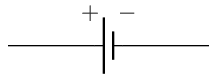
\includegraphics[width=25mm]{./phy1522/pile.png}
\end{center}

\hrulefill
\section{Constantes et conversions}
Permittivité du vide
\[ 	\epsilon_0 = \SI{8,85E-12}{{\farad}/{\meter}} \quad [\text{ou } \si{{\coulomb^2}/{(\newton\cdot\meter^2)}}] \]
\[	k = {1}/{4\pi\epsilon_0} = \SI{9,00E9}{\newton\cdot\meter^2/\kilogram^2}\]

Charge et masse de l'électron
\begin{gather*}
q_e = |e| = \SI{1,6E-19}{\coulomb}
\qquad m_e = \SI{9,11E-31}{\kilogram}
\end{gather*}

Masse volumique de l'eau
\[ \rho_\text{eau} = \SI{1000}{\kilogram/\meter^3} = \SI{1000}{\gram/\litre}  = \SI{1}{\kilogram/\litre} \]

Unités de volume
\[ \SI{1}{\litre} = \SI{1}{\deci\meter^3} =  \SI{1e-3}{\meter^3} \]

Unités de pression
\[ \SI{1}{\pascal} = \SI{1}{\newton/\meter^2} \]

Unités de travail
\[ \SI{1}{\joule} = \SI{1}{\kilo\pascal\cdot\litre} = \SI{1}{\newton\cdot\meter} = \SI{1}{\kilo\gram\cdot\metre^2/\sec^2} \]

Pression atmosphérique normale
\[ P_0 = \SI{1}{\text{atm}} = \SI{101,3}{\kilo\pascal}
= \SI{760}{\mmHg} \]

Nombre d'Avogadro
\[ N_A = \SI{6,02e23}{\mol^{-1}}\]

Constante des gaz parfaits
\[ R = \SI{8,314}{\joule/\mole\cdot\kelvin} \]

Constante de Bolzmann
\[ k = \SI{1,38E-23}{\joule/\kelvin} \]

Échelle de température
\[ T_K = T_C + \SI{273,15}{\kelvin} \]

Vitesse de la lumière
\[ c = \SI{3E8}{\meter/\second}  \]

\hrulefill


\section{Solides et fluides}

Masse volumique moyenne
\[ \rho = \frac{m}{V} \]

Modules d'élasticité, en général
\[ \text{module d'élasticité} = \frac{\text{contrainte}}{\text{déformation}} \]

Module de Young (traction des solides)
\[ E = \frac{\sigma}{\epsilon} 
= \frac{{F_\perp}/{A}}{{\Delta L}/{L_0}} 
\]

Module de rigidité (cisaillement des solides)
\[ G = \frac{\tau}{\gamma} 
= \frac{F_\parallel/A}{{\Delta x}/{h}} 
\]

Module de compressibilité (solides et fluides)
\[ K = - \left(\frac{\Delta P}{\Delta V / V} \right)\]

Pression [$\si{\pascal} = \si{\newton/\metre^2}$]
\[ P = \frac{F_\perp}{A} \]

Pression hydrostatique à la profondeur $h$
\[ P = P_0 + \rho gh \]

Principe d'Archimède : force de flottaison (poussée d'Archimède)
\[ F_p = \rho_\text{fluide} \, V_\text{déplacé} \, g \]

Équations de continuité (fluides ; écoulement laminaire stable)
\begin{align*}
	A_1 v_1 = A_2 v_2 \qquad &\text{(incompressible) [\si{\meter^3/\sec]}} \\
	\rho_1 A_1 v_1 = \rho_2 A_2 v_2 \qquad &\text{(compressible) [\si{\kilogram/\sec}]}
\end{align*}

Équation de Bernoulli
\[ P + \rho g y + \frac{1}{2}\rho v^2 = \text{constante} \]

\hrulefill


\section{Thermodynamique et gaz parfaits}

Principe zéro de la thermodynamique \\
\halfline
\begin{tabular}{@{\tableindent}p{0.8\linewidth}}
	Deux corps en équilibre thermique (même $T$) avec un troisième sont en équilibre thermique entre eux. \\
\end{tabular}
\halfline
	
Équation d'état d'un gaz parfait (de $N$ molécules ou $n$ moles)
\[ PV = Nkt = nRT \]

Dilation linéique (solides) et volumique (fluides et solides)
\[ \Delta L = \alpha L_0 \Delta T 
\qquad 
\Delta V = \beta V_0 \Delta T  \qquad  \beta = 3\alpha \text{ (solides)}
\]

Chaleur (transfert d'énergie)
\[ \Delta Q = mc\Delta T = nC\Delta T \]

Chaleur latente (changements de phase)
\[ \Delta Q = mL \]

Travail effectué \underline{par} un gaz dans un processus quasi statique (système toujours proche d'un état d'équilibre) [$\si{\joule} = \si{\kilo\pascal\cdot\litre}$]
\[ W = \int_{V_i}^{V_f} P\, dV \]

\tableindent (quasi statique $\Longrightarrow$ représentable sur un diagramme PV)
\halfline

Conventions de signe \\
\begin{tabular}{@{\tableindent}cl}
	$W_\text{gaz} > 0$ & le gaz fait du travail \\
	$W_\text{gaz} < 0$ & le gaz subit du travail \\
	$Q_\text{gaz} > 0$ & le gaz reçoit de la chaleur \\
	$Q_\text{gaz} < 0$ & le gaz émet de la chaleur \\
\end{tabular}
\halfline

Types de processus \\
\begin{tabular}{@{\tableindent}llcp{33mm}<{\raggedright}}
	isobare & $\Delta P=0$  & $ \Longrightarrow$ & $W=P\Delta V$  \\
	isochore & $\Delta V=0$  & $\Longrightarrow$ & $W=0$ \\
	isotherme & $\Delta T=0$ & $\Longrightarrow$& $W=nRT\ln(V_f/V_i)$ \scriptsize{(gaz parfait)}\\
	adiabatique & $Q=0$ & & \\
	%$\Longrightarrow$ & $\Delta U = -W$ \scriptsize{($1^\text{er}$ principe)} \\
\end{tabular}
\halfline

$1^\text{er}$ principe de la thermodynamique
\[ \Delta U = Q - W \]

Applications du $1^\text{er}$ principe de la thermodynamique \\
\renewcommand{\arraystretch}{1.2}
\begin{tabular}{@{\tableindent}m{24mm}<{\raggedright}p{18mm}<{\raggedright}cl}
	système isolé & $Q=0, W=0$ &$\Longrightarrow$ & $\Delta U = 0$ \\
	proc. cyclique & $\Delta U = 0$ &$\Longrightarrow$ & $Q=W$ \\
	proc. isochore & $W=0$ &$\Longrightarrow$ & $\Delta U = Q$ \\
	proc. adiabatique & $Q=0$ &$\Longrightarrow$ & $\Delta U = -W$ \\
	détente libre adiabatique & 
		$Q=0, W=0$ %\scriptsize{(expansion sans pousser un piston)}
		&$\Longrightarrow$ & $\Delta U = 0$ \\
\end{tabular}
\renewcommand{\arraystretch}{1}
\halfline

Autres propriétés d'un gaz parfait
\[ \Delta U = n C_V \Delta T  
\qquad 
C_P - C_V = R
\]

Processus adiabatique quasi statique pour un gaz parfait
\[ PV^\gamma = \text{constante} \qquad TV^{\gamma-1} = \text{constante}  \]
\[ \gamma = \frac{C_P}{C_V} > 1 
\qquad 
W = \frac{1}{\gamma - 1} (P_i V_i - P_f V_f) 
\]

\hrulefill

\section{Théorie cinétique}

Pression exercée par un gaz parfait
\[ P = \frac{1}{3} \rho v^2_\text{qm} \]

Vitesse quadratique moyenne des molécules
\[ v_\text{qm} = \sqrt{\overline{v^2}}
= \sqrt{\frac{3RT}{M}} 
= \sqrt{\frac{3kT}{m}} \]
\[ \overline{v^2_x} =  \overline{v^2_y} = \overline{v^2_z} = \frac{1}{3} v^2_\text{qm}  \]

Énergie cinétique moyenne de translation d'une molécule dans un gaz parfait
\[ K_\text{moy} = \frac{1}{2} mv^2_\text{qm} = \frac{3}{2} kT \]

Énergie interne d'un gaz parfait monoatomique
\[ U = \frac{3}{2} NkT = \frac{3}{2} nRT \]
\[ C_V = \frac{3}{2} R 
\qquad
C_P = \frac{5}{2} R
\qquad 
\gamma = \frac{C_P}{C_V} = \frac{5}{3} \]

Énergie interne d'un gaz diatomique
\begin{align*}
	U = \frac{5}{2} nRT \quad 
	C_V = \frac{5}{2} R  \quad 
	C_P = \frac{7}{2} R  \quad
	\gamma = \frac{7}{5} \quad &\text{ (rigide)} \\
	U = \frac{7}{2} nRT \quad 
	C_V = \frac{7}{2} R \quad 
	C_P = \frac{9}{2} R  \quad
	\gamma = \frac{9}{7} \quad &\text{ (non rigide)}
\end{align*}

\hrulefill

\section{Cycles, rendement et entropie}

Travail d'un moteur thermique
\[ W = |Q_C| - |Q_F| \]

Rendement thermique d'un moteur thermique
\[ \epsilon=\frac{W}{|Q_C|} = 1 - \frac{|Q_F|}{|Q_C|} \]

Coefficient d'amplification frigorifique et facteur calorifique
\[ \text{CAF} = \frac{|Q_F|}{W} \qquad
\text{FC} = \frac{|Q_C|}{W} \]

Rendement thermique du cycle de Carnot
\[ \epsilon= 1- \frac{T_F}{T_C} \]

$2^\text{e}$ principe de la thermodynamique
\[ \Delta S \geq 0 \]

\begin{tabular}{@{\tableindent}ll}
	processus réversible & $\Delta S_\text{isolé} = 0$ \\
	processus irréversible & $\Delta S_\text{isolé} > 0$ \\
\end{tabular}
\halfline

\hrulefill


\section{Rappel mathématique}

\subsection{Identités trigonométriques}
\halfline
\begin{multicols}{2}
\noindent
\[ \sin^2\theta +  \cos^2\theta = 1 \]
\begin{align*}
\cos 2\theta 
&=\cos^2\theta - \sin^2\theta \\
&=2\cos^2\theta - 1 \\
&=1  - 2\sin^2\theta 
\end{align*}
\[ \sin 2\theta  = 2\sin\theta\cos\theta  \]
\[ \sec^2\theta  = 1+ \tan^2\theta \]
\[ \csc^2\theta  = 1+ \cot^2\theta \]
\[ \tan 2\theta = \frac{2\tan\theta}{1-\tan^2\theta} \]
\[ \tan \theta = \pm\sqrt{\frac{1-\cos 2\theta}{1+\cos 2\theta}} = \frac{\sin\theta}{\cos\theta} \]
\end{multicols}
\[ \sin(A\pm B) = \sin A\cos B \pm \cos A\sin B\]
\[ \cos(A\pm B) = \cos A\cos B \mp \sin A\sin B\]

\subsection{Quelques dérivées}
\halfline
\begin{multicols}{2}
\noindent
\[ \deriv (ax^n) = nax^{n-1}\]
\[ \deriv (e^{ax}) = ae^{ax}\]
\[ \deriv (\ln ax) = \frac{a}{x} \]
\[ \deriv (\sin ax) = a\cos ax\]
\[ \deriv (\cos ax) = -a\sin ax\]
\[ \deriv (\tan ax) = a\sec^2 ax\]
\[ \deriv (\sec x) = \tan x \sec x \]
\[ \deriv (\cot x) = -a\csc^2 ax \]
\[ \deriv (\csc x) = -\cot x \csc x \]
\end{multicols}
\[ \deriv [f(x)\,g(x)] = f(x)g'(x) + g(x)f'(x)  \]
\[ \deriv \left[ \frac{f(x)}{g(x)} \right] = \frac{g(x)f'(x) - f(x)g'(x)}{[g(x)]^2}  \]
\[ \deriv [f(g(x))] = f'(g(x)) \, g'(x) \]

\subsection{Intégrales résolues}
\halfline
\begin{multicols}{2}
\noindent
\[ \int x^n \,dx =  \frac{x^{n+ 1}}{n+1} \quad (n\neq 1) \]
\[ \int e^{ax}\,dx = \frac{1}{a}e^{ax} \]
\[ \int \ln(ax) = x\ln(ax) - x \]
\[ \int \sin(ax)\,dx =-\frac{1}{a} \cos(ax) \]
\[ \int \cos(ax)\,dx =\frac{1}{a} \sin(ax) \]
\[ \int \sin^2(ax)\,dx = \frac{x}{2} - \frac{\sin(2ax)}{4a} \]
\[ \int \cos^2(ax)\,dx = \frac{x}{2} + \frac{\sin(2ax)}{4a} \]
%
\[ \int_a^b u\,dv = uv|_a^b - \int_a^b v\,du  \]
\end{multicols}

\extraline
Formes avec numérateur $dx$ 
\halfline
\begin{multicols}{2}
\noindent
\[ \int \frac{dx}{x} = \ln \lvert x \rvert \]
\[ \int \frac{dx}{a+bx} = \frac{1}{b}\ln\lvert a+bx\rvert \]
\[ \int \frac{dx}{x^2+a^2} = \frac{1}{a}\arctan\left(\frac{x}{a}\right) \]
\[\int \frac{dx}{\sqrt{x^2+a^2}} = \ln \lvert x + \sqrt{x^2+a^2} \rvert \]
\[ \int \frac{dx}{(x^2+a^2)^{3/2}} = \frac{x}{a^2\sqrt{x^2+a^2}} \]
\[ \int \frac{dx}{(a+bx)^2} = -\frac{1}{b(a+bx)} \]
\end{multicols}
%


\extraline
Formes avec numérateur $x\,dx$
\[ \int \frac{x\,dx}{(x^2 \pm a^2)^{1/2}} = \sqrt{x^2 \pm a^2} \]
\[\int \frac{x\,dx}{(x^2+a^2)^{3/2}} = -\frac{1}{\sqrt{x^2+a^2}} \]
\[ \int \frac{x\,dx}{(x^2+a^2)^n} = -\frac{1}{2(n-1)} \frac{1}{(x^2+a^2)^{n-1}} \quad (n>0)  \]
\[ \int \frac{x\,dx}{(a^2-bx)^{3/2}} = \frac{2x}{b\sqrt{a^2-bx}} + \frac{4\sqrt{a^2-bx}}{b^2} \]

%\extraline

Formes avec numérateur $x^2\,dx$
\[ \int \frac{x^2\,dx}{\sqrt{x^2+a^2}} =  \frac{u}{2}\sqrt{x^2+a^2} - \frac{a^2}{2}\ln(x+\sqrt{x^2+a^2}) \]
%
\[ \int \frac{x^2\,dx}{(x^2+a^2)^{3/2}} = -\frac{x}{\sqrt{x^2+a^2}} + \ln \lvert x + \sqrt{x^2+a^2} \rvert \]


\subsection{Autres formules}
Lois des logarithmes
\begin{gather*}
\log_a (xy) = \log_a x + \log_a y \\
 \log_a (x/y) = \log_a x - \log_a y \\
\log_a (x^r) = r\log_a x
\end{gather*}

Géométrie \\
\halfline
\begin{tabular}{@{\tableindent}ll@{}}
	Cercle & $C = 2\pi r $, $A =\pi r^2$ \\
	Sphère & $A = 4\pi r^2$, $V = \frac{4}{3}\pi r^3 $ \\
\end{tabular}
\extraline

Résolution d'une équation quadratique
\[ ax^2 + bx + c = 0 \Longrightarrow x = \frac{-b \pm \sqrt{b^2-4ac} }{2a} \]






\hrulefill


\scriptsize

\href{https://github.com/zhouluke/PhysicsFormulas}{Dactylographie}  \copyright\ 2022 Luke Zhou. \\
D'après le cours PHY 1522 Hiver 2022 de l'Université d'Ottawa. \\
\href{http://wch.github.io/latexsheet/}{Modèle de document}  \copyright\ 2014 Winston Chang.


\end{multicols}



\end{document}
